\documentclass{article}
\usepackage[utf8x]{inputenc}
\usepackage{graphicx}
\usepackage{tikz, amsmath, amssymb, bm, color}
\usepackage{geometry}
\usetikzlibrary{calc}
\usetikzlibrary{shapes,arrows}
\usepackage[disable, colorinlistoftodos]{todonotes}
\usepackage[american]{circuitikz}
\usepackage{pgfplots}
\usepackage{epstopdf}
\usepackage{listings}
\usepackage{subcaption}
\usepackage{mwe}
\usepackage{float}
\usepackage{cleveref}
\usepackage{ragged2e} % For text alignment


\newenvironment{s_itemize}{
\begin{itemize}
  \setlength{\itemsep}{0pt}
  \setlength{\parskip}{0pt}
  \setlength{\parsep}{0pt}
}{\end{itemize}}

\newenvironment{s_enumerate}{
\begin{enumerate}
  \setlength{\itemsep}{0pt}
  \setlength{\parskip}{0pt}
  \setlength{\parsep}{0pt}
}{\end{enumerate}}

\begin{document}

\section*{Hardware Characterization}

\subsection*{Required measurements}
\begin{lstlisting}
http://ra.ziti.uni-heidelberg.de/pages/student_work/
seminar/ws0304/richard_sohnius/praesentation.pdf
\end{lstlisting}


Transition times. Characterized and measured between $30\,\%$ and $70\,\%$. Standardized reporting between $10\,\%$ and $90\,\%$.


\begin{s_itemize} 
\item area
\item power
\item timing contstraints (setup/Hold time, recovery/removal time)
\item propagation delay time
\item input capacitance
\end{s_itemize} 
%
%
\textbf{Power}:
\begin{s_itemize}
	\item Dynamic power (switching power)
	\item Static power (leakage power)
	\item Passive power (internal power. power used by sequential cells when inputs change without output change)
\end{s_itemize}
%
%
\textbf{Delay}:
\begin{lstlisting}
https://www.csee.umbc.edu/~cpatel2/links/641/slides/lect05_LIB.pdf
\end{lstlisting}

\begin{s_itemize}
\item sum of intrinsic delay, slope delay, transition delay and connect delay
\item intrinsic delay is fixed value independent of surroundings
\item slope delay is produced by the slew of the input signal
\item transition delay is the time required to change the capacitance of the next stage input pins
\item connect delay is delay caused by the wire between output and next input pins
\end{s_itemize}

Delay model of Liberate (.lib) is the CMOS Non-Linear Delay Model.
\begin{s_itemize}
\item Delay and transition time are modeled as function of Input slew and Output load
\item Data is stored in a 2D LUT (look-up table)
\item Intermediate values are interpolated
\item Data points are usually not equidistant
\end{s_itemize}




\subsection*{solutions}
feedback loop with a counter?
\section*{Solutions}

Timing: use frequency divider (Alex's grey counter) and a ring oscillator
can characterize 64 cells? only needs to change a single cell and wait for a while.\\
\\
Power: simply switch of the counter, let the ring oscillator run and measure the power. The only changes are within the ring oscillator, so over time the power gets more precise.\\
\\
Area is of no concern

\clearpage
\section*{Testbenches}
%\subsection*{Low Voltage Differential Signaling (LVDS) Receiver}
\subsection*{Numerically Controlled Oscillator}
Numerically controlled oscillator

\begin{lstlisting}
Clock Source Selection (pick a clock)
 ||
 \/
Accumulator        <== increment value (1 to 65535)
(20 bits counter, remainder flows over to next round)
 ||
 \/
Output Control
\end{lstlisting}

\subsection*{Time to Digital Converter (TDC)}


\begin{figure}[H]
\centering
\tikzstyle{dot} = [draw,shape=circle,fill=black, scale =.3]
\begin{tikzpicture}

% DFF Block
\draw  (-1.5,1) rectangle (0,-0.5);
\draw (-1.5,-0.125) to (-1.25,-0.25) to (-1.5,-0.375);
\node at (-1.25,0.75) {$D$};
\node at (-0.25,0.25) {$Q$};

% DFF Block
\draw  (0.75,1) rectangle (2.25,-0.5);
\draw (0.75,-0.125) to (1,-0.25) to (0.75,-0.375);
\node at (1,0.75) {$D$};
\node at (2,0.25) {$Q$};

% DFF Block
\draw  (3,1) rectangle (4.5,-0.5);
\draw (3,-0.125) to (3.25,-0.25) to (3,-0.375);
\node at (3.25,0.75) {$D$};
\node at (4.25,0.25) {$Q$};

% buffer gate
\draw (0,0) node [buffer, scale=.75] (buf1) at (-0.75,1.75) {};
\draw (buf1.in) -- (-2,1.75);
\draw (-1.75,1.75)|-(-1.5,0.75);
\node [dot] at (-1.75,1.75) {};

% buffer gate
\draw (0,0) node [buffer, scale=.75] (buf2) at (1.5,1.75) {};
\draw (buf2.in) -- (buf1.out);
\draw (0.5,1.75)|-(0.75,0.75);
\node [dot] at (0.5,1.75) {};

% buffer gate
\draw (0,0) node [buffer, scale=.75] (buf3) at (3.75,1.75) {};
\draw (buf3.in) -- (buf2.out);
\draw (buf3.out) -- (5,1.75);
\draw (2.75,1.75)|-(3,0.75);
\node [dot] at (2.75,1.75) {};

%ref(t)
\draw (-2,-1) -- (5,-1);
\draw (-1.75,-1)|-(-1.5,-0.25);
\node [dot] at (-1.75,-1) {};
\draw (0.5,-1)|-(0.75,-0.25);
\node [dot] at (0.5,-1) {};
\draw (2.75,-1)|-(3,-0.25);
\node [dot] at (2.75,-1) {};

%error
\draw (0,0.25) -| (0.25,-1.25) -| (4.5,-1.5);
\draw (2.25,0.25) -| (2.5,-1.375) -| (4.65,-1.5);
\draw (4.5,0.25) -| (4.75,-1.5);
\draw  (4,-1.5) rectangle (5.25,-2) node[pos=.5]{adder};
\draw (4.625,-2) -- (4.625,-2.25);

% labels
\node [anchor=east] at (-2,1.75) {div$(t)$};
\node [anchor=east] at (-2,-1) {ref$(t)$};
\node [anchor=north] at (4.625,-2.25) {err$(t)$};
\end{tikzpicture}
\caption{TDC}
\label{tkz:TDC}
\end{figure}
\subsection*{Phase Detector}
The phase detector  produces a 1 between the time the reference signal switches to a one, and the divider switches to a one.


\begin{figure}[H]
\centering
\tikzstyle{dot} = [draw,shape=circle,fill=black, scale =.3]
\begin{tikzpicture}

% DFF Block
\draw  (-1.5,1) rectangle (0,-0.5);
\draw (-1.5,-0.125) to (-1.25,-0.25) to (-1.5,-0.375);
\node at (-1.25,0.75) {$D$};
\node at (-0.25,0.25) {$Q$};

% DFF Block
\draw  (-1.5,-1.5) rectangle (0,-3);
\draw (-1.5,-2.625) to (-1.25,-2.75) to (-1.5,-2.875);
\node at (-1.25,-1.75) {$D$};
\node at (-0.25,-2.25) {$Q$};

% and gate
\draw (0,0) node [and port, rotate=180] (and1) at (0.5,-1) {};
\draw (0,-2.25) -| (and1.in 1);
\draw (0,.25) -| (and1.in 2);

% reset
\draw (-0.75,-0.5) |- (and1.out);
\draw (-0.75, -1) -- (-0.75, -1.5);
\node [dot] at (-0.75,-1) {};
\node [anchor=east] at (-0.75,-1) {reset};

% 1's
\draw(-1.75,0.75) -- (-1.5,0.75);
\node [anchor=east] at (-1.75,0.75) {$1$};
\draw(-1.75,-1.75) -- (-1.5,-1.75);
\node [anchor=east] at (-1.75,-1.75) {$1$};

% signals
\draw(-1.75,-0.25) -- (-1.5,-0.25);
\node [anchor=east] at (-1.75,-0.25) {ref$(t)$};
\draw(-1.75,-2.75) -- (-1.5,-2.75);
\node [anchor=east] at (-1.75,-2.75) {div$(t)$};

% error
\draw(1.875,.25) -- (2.25,0.25);
\node [anchor=south] at (1.9,0.25) {error$(t)$};
\node[dot] at (1.885,.25) {};
\end{tikzpicture}
\caption{Phase detector}
\label{tkz:phaseDetector}
\end{figure}

\subsection*{Digitally controlled oscillator}
Uses digitally controlled switches to change the output load
\subsection*{Grey Counter}
8-bit grey counter designed with Alex
\subsection*{Digital Divider}


\begin{figure}[H]
\centering
\tikzstyle{dot} = [draw,shape=circle,fill=black, scale =.3]
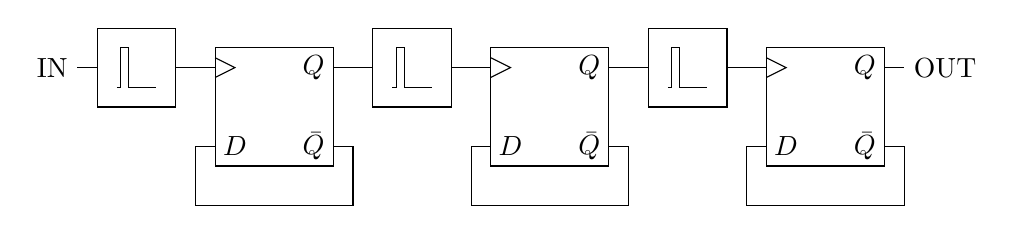
\begin{tikzpicture}
%%% entire block
% DFF Block
\draw  (-1.5,1) rectangle (0,-0.5);
\draw (-1.5,0.875) to (-1.25,0.75) to (-1.5,0.625);
\node at (-1.25,-0.25) {$D$};
\node at (-0.25,0.75) {$Q$};
\node at (-0.25,-0.25) {$\bar{Q}$};

% connections
\draw (0,-0.25) -| (0.25,-1) -- (-1.75,-1) |- (-1.5,-0.25);
\draw (-1.5,0.75) -- (-2,0.75);
\draw (-3,0.75) -- (-3.25,0.75);

% pulse generator
\draw (-2.75,0.5) -| (-2.7,1) -| (-2.6,0.5) -- (-2.25,0.5);
\draw  (-3,1.25) rectangle (-2,0.25);

%%% entire block
% DFF Block
\draw  (2,1) rectangle (3.5,-0.5);
\draw (2,0.875) to (2.25,0.75) to (2,0.625);
\node at (2.25,-0.25) {$D$};
\node at (3.25,0.75) {$Q$};
\node at (3.25,-0.25) {$\bar{Q}$};

% connections
\draw (3.5,-0.25) -| (3.75,-1) -- (1.75,-1) |- (2,-0.25);
\draw (2,0.75) -- (1.5,0.75);
\draw (0.5,0.75) -- (0,0.75);

% pulse generator
\draw (0.75,0.5) -| (0.8,1) -| (0.9,0.5) -- (1.25,0.5);
\draw  (0.5,1.25) rectangle (1.5,0.25);

%%% entire block
% DFF Block
\draw  (5.5,1) rectangle (7,-0.5);
\draw (5.5,0.875) to (5.75,0.75) to (5.5,0.625);
\node at (5.75,-0.25) {$D$};
\node at (6.75,0.75) {$Q$};
\node at (6.75,-0.25) {$\bar{Q}$};

% connections
\draw (7,-0.25) -| (7.25,-1) -- (5.25,-1) |- (5.5,-0.25);
\draw (5.5,0.75) -- (5,0.75);
\draw (4,0.75) -- (3.5,0.75);

% pulse generator
\draw (4.25,0.5) -| (4.3,1) -| (4.4,0.5) -- (4.75,0.5);
\draw  (4,1.25) rectangle (5,0.25);


%in and out
\draw(7,0.75) -- (7.25,0.75);
\node [anchor=east] at (-3.25,0.75) {IN};
\node [anchor=west]  at (7.25,0.75) {OUT};
\end{tikzpicture}

\caption{Digital divider}
\label{tkz:digitalDivider}
\end{figure}
\subsection*{4-bit Multiplexer and Demultiplexer}

\begin{figure}[H]
\centering
\tikzstyle{dot} = [draw,shape=circle,fill=black, scale =.3]
\begin{tikzpicture}

% and row
\draw (3,3) node [and port, scale=.75, rotate = -90] (and1) at (3,3) {};
\draw (1.5,3) node [and port, scale=.75, rotate = -90] (and2) at (2,3) {};
\draw (1.5,3) node [and port, scale=.75, rotate = -90] (and3) at (1,3) {};
\draw (0,3) node [and port, scale=.75, rotate = -90] (and4) at (0,3) {};

% or with connections
\draw (3,3) node [or port, scale=.75, rotate = -90] (or3) at (1.5,1.75) {};
\draw
(and2.out) -| (1.58,2.45)
(and3.out) -| (1.42,2.45)
(and4.out) -- (0,2.8) -| (or3.in 2)
(and1.out) -- (3,2.8) -| (or3.in 1);

% selection lines lines
\draw (3,3) node [not port, scale=.35] (buf1) at (-0.75,4.75) {};
\draw (3,3) node [not port, scale=.35] (buf2) at (-0.75,4.25) {};
\draw (-1,5) |- (buf1.in);
\draw (-1.125,5) -| (and3.in 1);
\draw (buf1.out) -| (and1.in 1);
\draw (-1,4.5) |- (buf2.in);
\draw (-1.125,4.5) -| (and2.in 2);
\draw (buf2.out) -| (and1.in 2);

%selection connection
\draw (2.2,4.75)--(and2.in 1); \node[dot] at (2.2,4.75) {};
\draw (0.2,5)--(and4.in 1); \node[dot] at (0.2,5) {};
\draw (0.79,4.25)--(and3.in 2); \node[dot] at (0.79,4.25) {};
\draw (-0.22,4.5)--(and4.in 2); \node[dot] at (-0.22,4.5) {};

%source
\draw (1.5,3) node [buffer,scale = .6, rotate = -90] (buf) at (1.5,5.75) {};
\draw
(buf.out) -| (0,3.88)
(buf.out) -| (1,3.88)
(buf.out) -| (2,3.88)
(buf.out) -| (3,3.88);

% labels
\node[anchor=east] at (-1.125,5) {sel[0]};
\node[anchor=east] at (-1.125,4.5) {sel[1]};
\node[anchor=south] at (1.5,6.125) {IN};
\node at (1.5,1.5) {OUT};

% and row
\draw (9.75,3) node [and port, scale=.75, rotate = -90] (and1) at (9.75,3) {};
\draw (8.25,3) node [and port, scale=.75, rotate = -90] (and2) at (8.75,3) {};
\draw (8.25,3) node [and port, scale=.75, rotate = -90] (and3) at (7.75,3) {};
\draw (6.75,3) node [and port, scale=.75, rotate = -90] (and4) at (6.75,3) {};

% selection lines lines
\draw (9.75,3) node [not port, scale=.35] (buf1) at (6,4.75) {};
\draw (9.75,3) node [not port, scale=.35] (buf2) at (6,4.25) {};
\draw (5.75,5) |- (buf1.in);
\draw (5.625,5) -| (and3.in 1);
\draw (buf1.out) -| (and1.in 1);
\draw (5.75,4.5) |- (buf2.in);
\draw (5.625,4.5) -| (and2.in 2);
\draw (buf2.out) -| (and1.in 2);

%selection connection
\draw (8.95,4.75)--(and2.in 1); \node[dot] at (8.95,4.75) {};
\draw (6.95,5)--(and4.in 1); \node[dot] at (6.95,5) {};
\draw (7.54,4.25)--(and3.in 2); \node[dot] at (7.54,4.25) {};
\draw (6.53,4.5)--(and4.in 2); \node[dot] at (6.53,4.5) {};

%source
\draw (8.25,3) node [buffer,scale = .6, rotate = -90] (buf) at (8.25,5.75) {};
\draw
(buf.out) -| (6.75,3.88)
(buf.out) -| (7.75,3.88)
(buf.out) -| (8.75,3.88)
(buf.out) -| (9.75,3.88);

%outputs
\draw (and4.out) -- (6.75,1.75); \node at (6.75,1.5) {\tiny{OUT[0]}};
\draw (and3.out) -- (7.75,1.75); \node at (7.75,1.5) {\tiny{OUT[1]}};
\draw (and2.out) -- (8.75,1.75); \node at (8.75,1.5) {\tiny{OUT[2]}};
\draw (and1.out) -- (9.75,1.75); \node at (9.75,1.5) {\tiny{OUT[3]}};

% labels
\node[anchor=east] at (5.625,5) {sel[0]};
\node[anchor=east] at (5.625,4.5) {sel[1]};
\node[anchor=south] at (8.25,6.125) {IN};
\end{tikzpicture}


\caption{MUX}
\label{tkz:MUX}
\end{figure}
\subsection*{Changable Ring Oscillator}

\begin{figure}[H]
\centering
\tikzstyle{dot} = [draw,shape=circle,fill=black, scale =.3]
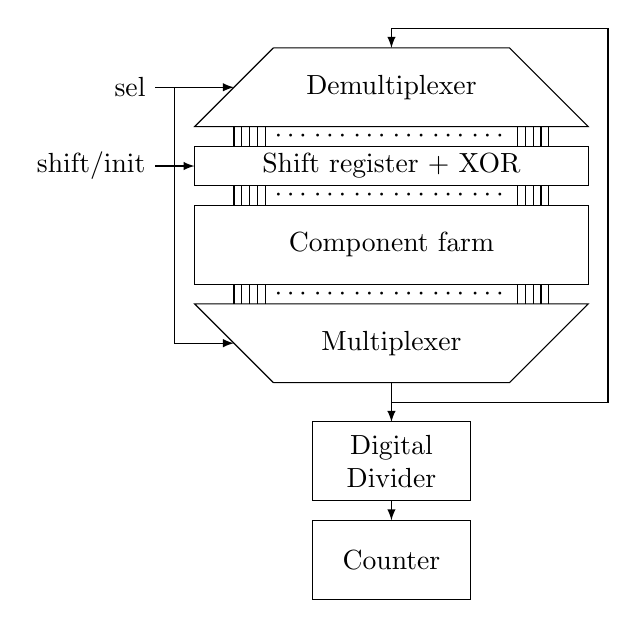
\begin{tikzpicture}
% Multiplexer and demultiplexer
\draw (1.5,6.5) -- (4.5,6.5) -- (5.5,5.5) -- (0.5,5.5) --  (1.5,6.5);
\node at (3,6) {Demultiplexer};
\draw (1.5,2.25) -- (4.5,2.25) -- (5.5,3.25) -- (0.5,3.25) --  (1.5,2.25);
\node at (3,2.75) {Multiplexer};

%components with connects
\draw  (0.5,5.25) rectangle (5.5,4.75) node[pos=.5]{Shift register + XOR};
\draw 
(1,4.5) -- (1,4.75)
(1.1,4.5) -- (1.1,4.75)
(1.2,4.5) -- (1.2,4.75)
(1.3,4.5) -- (1.3,4.75)
(1.4,4.5) -- (1.4,4.75);
\draw 
(4.6,4.5) -- (4.6,4.75)
(4.7,4.5) -- (4.7,4.75)
(4.8,4.5) -- (4.8,4.75)
(4.9,4.5) -- (4.9,4.75)
(5,4.5) -- (5,4.75);
\node at (1.75,4.625) {$\cdots$};
\node at (2.25,4.625) {$\cdots$};
\node at (2.75,4.625) {$\cdots$};
\node at (3.25,4.625) {$\cdots$};
\node at (3.75,4.625) {$\cdots$};
\node at (4.25,4.625) {$\cdots$};


\draw  (0.5,4.5) rectangle (5.5,3.5) node[pos=.5]{Component farm};
\draw 
(1,5.25) -- (1,5.5)
(1.1,5.25) -- (1.1,5.5)
(1.2,5.25) -- (1.2,5.5)
(1.3,5.25) -- (1.3,5.5)
(1.4,5.25) -- (1.4,5.5);
\draw 
(4.6,5.25) -- (4.6,5.5)
(4.7,5.25) -- (4.7,5.5)
(4.8,5.25) -- (4.8,5.5)
(4.9,5.25) -- (4.9,5.5)
(5,5.25) -- (5,5.5);
\node at (1.75,5.375) {$\cdots$};
\node at (2.25,5.375) {$\cdots$};
\node at (2.75,5.375) {$\cdots$};
\node at (3.25,5.375) {$\cdots$};
\node at (3.75,5.375) {$\cdots$};
\node at (4.25,5.375) {$\cdots$};
\draw 
(1,3.25) -- (1,3.5)
(1.1,3.25) -- (1.1,3.5)
(1.2,3.25) -- (1.2,3.5)
(1.3,3.25) -- (1.3,3.5)
(1.4,3.25) -- (1.4,3.5);
\draw 
(4.6,3.25) -- (4.6,3.5)
(4.7,3.25) -- (4.7,3.5)
(4.8,3.25) -- (4.8,3.5)
(4.9,3.25) -- (4.9,3.5)
(5,3.25) -- (5,3.5);
\node at (1.75,3.375) {$\cdots$};
\node at (2.25,3.375) {$\cdots$};
\node at (2.75,3.375) {$\cdots$};
\node at (3.25,3.375) {$\cdots$};
\node at (3.75,3.375) {$\cdots$};
\node at (4.25,3.375) {$\cdots$};

% feedback, counter and digital divider
\draw  (2,0.5) rectangle (4,-0.5) node[pos=.5, align=center]{Counter};
\draw [>=latex, ->](3,0.75) -- (3,0.5);
\draw  (2,1.75) rectangle (4,0.75) node[pos=.5, align=center]{Digital\\Divider};
\draw [>=latex, ->](3,2.25) -- (3,1.75);
\draw [>=latex, ->](3,2) -- (5.75,2) -- (5.75,6.75) -| (3,6.5);

%enable and select
\draw [>=latex, ->] (0.25,6) |- (1,2.75);
\draw [>=latex, ->] (0,6) -- (1,6);
\node [anchor=east] at (0,6) {sel};
\draw [>=latex, ->] (0,5) -- (0.5,5);
\node [anchor=east] at (0,5) {shift/init};
\end{tikzpicture}

\caption{Changable Ring Oscillator}
\label{tkz:changableRingOscillator}
\end{figure}

\begin{figure}[H]
\centering
\tikzstyle{dot} = [draw,shape=circle,fill=black, scale =.3]
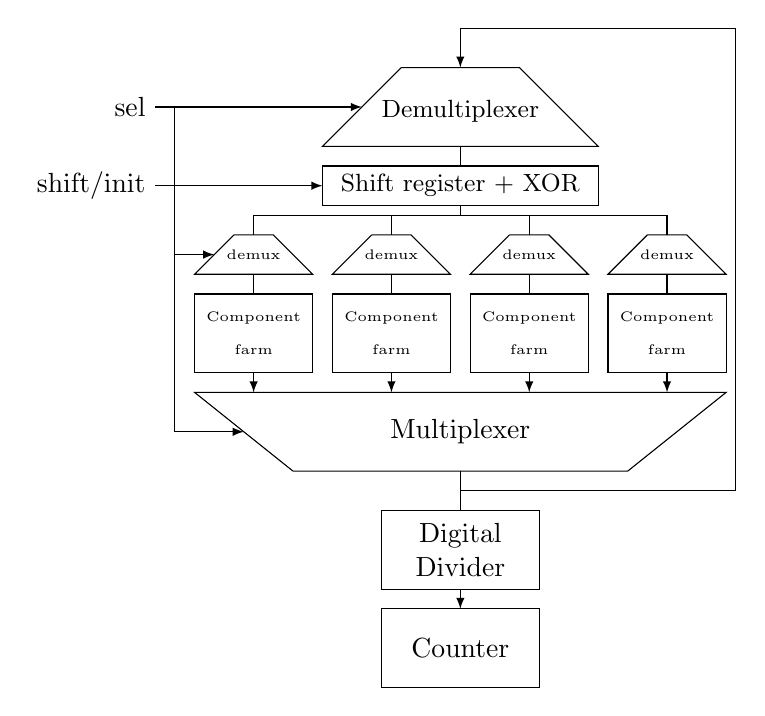
\begin{tikzpicture}
% Multiplexer and demultiplexer
\draw (2.625,8.25) -- (4.125,8.25) -- (5.125,7.25) -- (1.625,7.25) --  (2.625,8.25);
\node at (3.375,7.7) {\small{Demultiplexer}};
\draw (1.25,3.125) -- (5.5,3.125) -- (6.75,4.125) -- (0,4.125) --  (1.25,3.125);
\node at (3.375,3.625) {Multiplexer};

%shift register with connects
\draw  (1.625,7) rectangle (5.125,6.5) node[pos=.5]{\small{Shift register + XOR}};
\draw [>=latex, -](3.375,6.5) |- (0.75,6.375) -- (0.75,6.125);
\draw [>=latex, -](3.375,6.375) -| (6,6.125);
\draw [>=latex, -](4.25,6.375) -- (4.25,6.125);
\draw [>=latex, -](2.5,6.375) -- (2.5,6.125);

% component farm piece
\draw  (0,5.375) rectangle (1.5,4.375) node[pos=.5, align = center]{\tiny{Component}\\\tiny{farm}};
\draw (0.5,6.125) -- (1,6.125) -- (1.5,5.625) -- (0,5.625) --  (0.5,6.125);
\draw [>=latex, -] (0.75,5.625) -- (0.75,5.375);
\draw [>=latex, ->] (0.75,4.375) -- (0.75,4.125);
\node at (0.75,5.875) {\tiny{demux}};

% component farm piece
\draw  (1.75,5.375) rectangle (3.25,4.375) node[pos=.5, align = center]{\tiny{Component}\\\tiny{farm}};
\draw (2.25,6.125) -- (2.75,6.125) -- (3.25,5.625) -- (1.75,5.625) --  (2.25,6.125);
\draw [>=latex, -] (2.5,5.625) -- (2.5,5.375);
\draw [>=latex, ->] (2.5,4.375) -- (2.5,4.125);
\node at (2.5,5.875) {\tiny{demux}};

% component farm piece
\draw  (3.5,5.375) rectangle (5,4.375) node[pos=.5, align = center]{\tiny{Component}\\\tiny{farm}};
\draw (4,6.125) -- (4.5,6.125) -- (5,5.625) -- (3.5,5.625) --  (4,6.125);
\draw [>=latex, -] (4.25,5.625) -- (4.25,5.375);
\draw [>=latex, ->] (4.25,4.375) -- (4.25,4.125);
\node at (4.25,5.875) {\tiny{demux}};

% component farm piece
\draw  (5.25,5.375) rectangle (6.75,4.375) node[pos=.5, align = center]{\tiny{Component}\\\tiny{farm}};
\draw (5.75,6.125) -- (6.25,6.125) -- (6.75,5.625) -- (5.25,5.625) --  (5.75,6.125);
\draw [>=latex, -] (6,5.625) -- (6,5.375);
\draw [>=latex, ->] (6,4.375) -- (6,4.125);
\node at (6,5.875) {\tiny{demux}};

% feedback, counter and digital divider
\draw  (2.375,1.375) rectangle (4.375,0.375) node[pos=.5, align=center]{Counter};
\draw [>=latex, ->](3.375,1.625) -- (3.375,1.375);
\draw  (2.375,2.625) rectangle (4.375,1.625) node[pos=.5, align=center]{Digital\\Divider};
\draw [>=latex, -](3.375,3.125) -- (3.375,2.625);
\draw [>=latex, ->](3.375,2.875) -- (6.875,2.875) -- (6.875,8.75) -| (3.375,8.25);

%enable and select
\draw [>=latex, ->] (-0.25,7.75) |- (0.625,3.625);
\draw [>=latex, ->] (-0.5,7.75) -- (2.125,7.75);
\node [anchor=east] at (-0.5,7.75) {sel};
\draw [>=latex, ->] (-0.5,6.75) -- (1.625,6.75);
\node [anchor=east] at (-0.5,6.75) {shift/init};

\draw[>=latex, -] (3.375,7.25) -- (3.375,7);
\draw[>=latex, ->] (-0.25,5.875) -- (0.25,5.875);

\end{tikzpicture}

\caption{Changable Ring Oscillator 2}
\label{tkz:changableRingOscillator2}
\end{figure}



\begin{figure}[H]
\centering
\tikzstyle{dot} = [draw,shape=circle,fill=black, scale =.3]
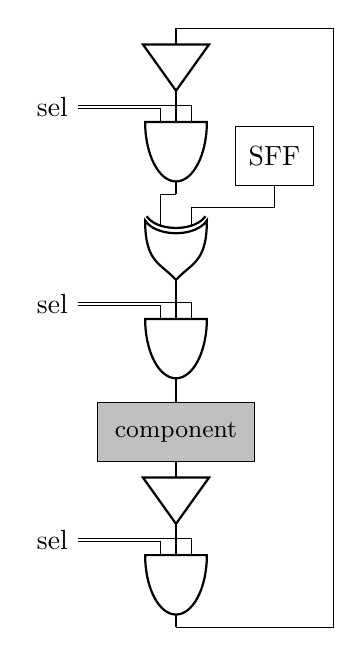
\begin{tikzpicture}
% Buffer
\draw (3,2.75) node [buffer, scale=.6, rotate = -90] (buf1) at (3,3) {};

% DEMUX
\draw (3,2.75) node [and port, scale=.7, rotate = -90] (and1) at (3,1.5) {};
\draw
(buf1.out) -- (3,2.3)
(1.75,2.52) -| (and1.in 1)
(1.75,2.48) -| (and1.in 2);
\node [anchor=east] at (1.75,2.5) {sel};

% Shift register + XOR
\draw (3,2.75) node [xor port, scale=.7, rotate = -90] (xor1) at (3,0.25) {};
\draw  (3.75,2.25) rectangle (4.75,1.5) node[pos=.5]{SFF};
\draw 
(and1.out) -| (xor1.in 2)
(4.25,1.5) |- (xor1.in 1)
;

% DEMUX
\draw (3,2.75) node [and port, scale=.7, rotate = -90] (and2) at (3,-1) {};
\draw
(xor1.out) -- (3,-0.2)
(1.75,0.02) -| (and2.in 1)
(1.75,-0.02) -| (and2.in 2);
\node [anchor=east] at (1.75,0) {sel};

% actual component
\draw [fill=lightgray] (2,-1.25) rectangle (4,-2) node[pos=.5]{\small{component}};
\draw (and2.out) -- (3,-1.25);

% MUX
\draw (3,2.75) node [buffer, scale=.6, rotate = -90] (buf2) at (3,-2.5) {};
\draw (3,-2) -- (buf2.in);
\draw (3,2.75) node [and port, scale=.7, rotate = -90] (and3) at (3,-4) {};
\draw
(3,-3.19) -- (buf2.out)
(1.75,-2.98) -| (and3.in 1)
(1.75,-3.02) -| (and3.in 2);
\node [anchor=east] at (1.75,-3) {sel};

%loop
\draw (and3.out)-| (5,3.5) -| (buf1.in);
\end{tikzpicture}
\caption{critical path of dynamic ring oscillator}
\label{tkz:criticalPath}
\end{figure}
\end{document}



